\documentclass[1p]{elsarticle_modified}
%\bibliographystyle{elsarticle-num}

%\usepackage[colorlinks]{hyperref}
%\usepackage{abbrmath_seonhwa} %\Abb, \Ascr, \Acal ,\Abf, \Afrak
\usepackage{amsfonts}
\usepackage{amssymb}
\usepackage{amsmath}
\usepackage{amsthm}
\usepackage{scalefnt}
\usepackage{amsbsy}
\usepackage{kotex}
\usepackage{caption}
\usepackage{subfig}
\usepackage{color}
\usepackage{graphicx}
\usepackage{xcolor} %% white, black, red, green, blue, cyan, magenta, yellow
\usepackage{float}
\usepackage{setspace}
\usepackage{hyperref}

\usepackage{tikz}
\usetikzlibrary{arrows}

\usepackage{multirow}
\usepackage{array} % fixed length table
\usepackage{hhline}

%%%%%%%%%%%%%%%%%%%%%
\makeatletter
\renewcommand*\env@matrix[1][\arraystretch]{%
	\edef\arraystretch{#1}%
	\hskip -\arraycolsep
	\let\@ifnextchar\new@ifnextchar
	\array{*\c@MaxMatrixCols c}}
\makeatother %https://tex.stackexchange.com/questions/14071/how-can-i-increase-the-line-spacing-in-a-matrix
%%%%%%%%%%%%%%%

\usepackage[normalem]{ulem}

\newcommand{\msout}[1]{\ifmmode\text{\sout{\ensuremath{#1}}}\else\sout{#1}\fi}
%SOURCE: \msout is \stkout macro in https://tex.stackexchange.com/questions/20609/strikeout-in-math-mode

\newcommand{\cancel}[1]{
	\ifmmode
	{\color{red}\msout{#1}}
	\else
	{\color{red}\sout{#1}}
	\fi
}

\newcommand{\add}[1]{
	{\color{blue}\uwave{#1}}
}

\newcommand{\replace}[2]{
	\ifmmode
	{\color{red}\msout{#1}}{\color{blue}\uwave{#2}}
	\else
	{\color{red}\sout{#1}}{\color{blue}\uwave{#2}}
	\fi
}

\newcommand{\Sol}{\mathcal{S}} %segment
\newcommand{\D}{D} %diagram
\newcommand{\A}{\mathcal{A}} %arc


%%%%%%%%%%%%%%%%%%%%%%%%%%%%%5 test

\def\sl{\operatorname{\textup{SL}}(2,\Cbb)}
\def\psl{\operatorname{\textup{PSL}}(2,\Cbb)}
\def\quan{\mkern 1mu \triangleright \mkern 1mu}

\theoremstyle{definition}
\newtheorem{thm}{Theorem}[section]
\newtheorem{prop}[thm]{Proposition}
\newtheorem{lem}[thm]{Lemma}
\newtheorem{ques}[thm]{Question}
\newtheorem{cor}[thm]{Corollary}
\newtheorem{defn}[thm]{Definition}
\newtheorem{exam}[thm]{Example}
\newtheorem{rmk}[thm]{Remark}
\newtheorem{alg}[thm]{Algorithm}

\newcommand{\I}{\sqrt{-1}}
\begin{document}

%\begin{frontmatter}
%
%\title{Boundary parabolic representations of knots up to 8 crossings}
%
%%% Group authors per affiliation:
%\author{Yunhi Cho} 
%\address{Department of Mathematics, University of Seoul, Seoul, Korea}
%\ead{yhcho@uos.ac.kr}
%
%
%\author{Seonhwa Kim} %\fnref{s_kim}}
%\address{Center for Geometry and Physics, Institute for Basic Science, Pohang, 37673, Korea}
%\ead{ryeona17@ibs.re.kr}
%
%\author{Hyuk Kim}
%\address{Department of Mathematical Sciences, Seoul National University, Seoul 08826, Korea}
%\ead{hyukkim@snu.ac.kr}
%
%\author{Seokbeom Yoon}
%\address{Department of Mathematical Sciences, Seoul National University, Seoul, 08826,  Korea}
%\ead{sbyoon15@snu.ac.kr}
%
%\begin{abstract}
%We find all boundary parabolic representation of knots up to 8 crossings.
%
%\end{abstract}
%\begin{keyword}
%    \MSC[2010] 57M25 
%\end{keyword}
%
%\end{frontmatter}

%\linenumbers
%\tableofcontents
%
\newcommand\colored[1]{\textcolor{white}{\rule[-0.35ex]{0.8em}{1.4ex}}\kern-0.8em\color{red} #1}%
%\newcommand\colored[1]{\textcolor{white}{ #1}\kern-2.17ex	\textcolor{white}{ #1}\kern-1.81ex	\textcolor{white}{ #1}\kern-2.15ex\color{red}#1	}

{\Large $\underline{12a_{0235}~(K12a_{0235})}$}

\setlength{\tabcolsep}{10pt}
\renewcommand{\arraystretch}{1.6}
\vspace{1cm}\begin{tabular}{m{100pt}>{\centering\arraybackslash}m{274pt}}
\multirow{5}{120pt}{
	\centering
	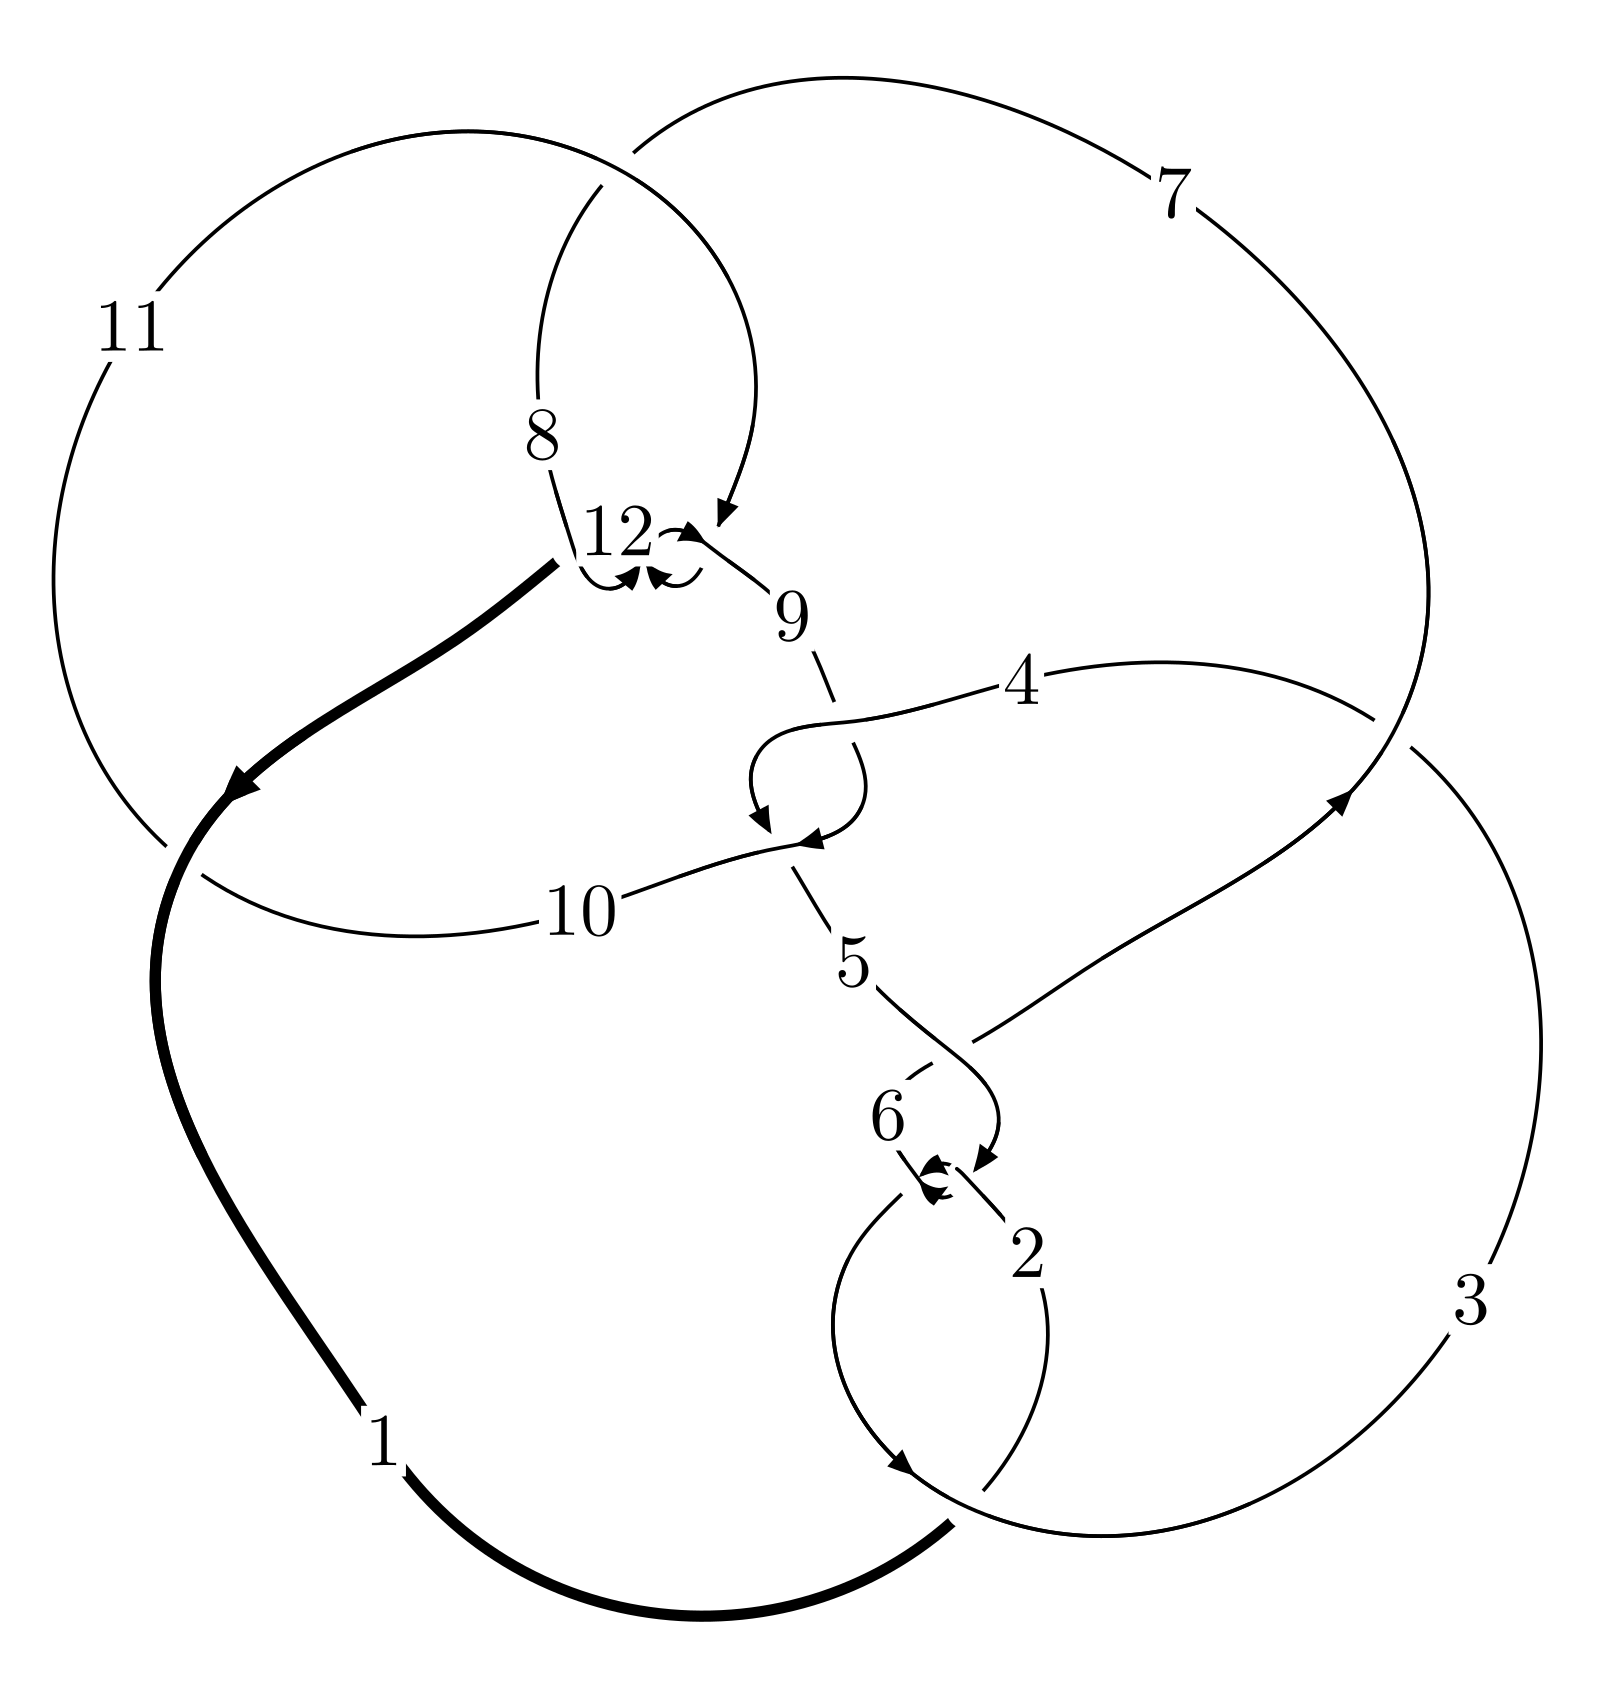
\includegraphics[width=112pt]{../../../GIT/diagram.site/Diagrams/png/1036_12a_0235.png}\\
\ \ \ A knot diagram\footnotemark}&
\allowdisplaybreaks
\textbf{Linearized knot diagam} \\
\cline{2-2}
 &
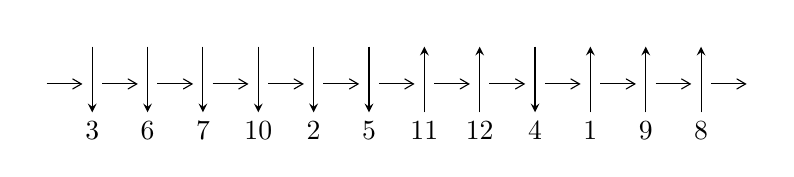
\begin{tikzpicture}[x=20pt, y=17pt]
	% nodes
	\node (C0) at (0, 0) {};
	\node (C1) at (1, 0) {};
	\node (C1U) at (1, +1) {};
	\node (C1D) at (1, -1) {3};

	\node (C2) at (2, 0) {};
	\node (C2U) at (2, +1) {};
	\node (C2D) at (2, -1) {6};

	\node (C3) at (3, 0) {};
	\node (C3U) at (3, +1) {};
	\node (C3D) at (3, -1) {7};

	\node (C4) at (4, 0) {};
	\node (C4U) at (4, +1) {};
	\node (C4D) at (4, -1) {10};

	\node (C5) at (5, 0) {};
	\node (C5U) at (5, +1) {};
	\node (C5D) at (5, -1) {2};

	\node (C6) at (6, 0) {};
	\node (C6U) at (6, +1) {};
	\node (C6D) at (6, -1) {5};

	\node (C7) at (7, 0) {};
	\node (C7U) at (7, +1) {};
	\node (C7D) at (7, -1) {11};

	\node (C8) at (8, 0) {};
	\node (C8U) at (8, +1) {};
	\node (C8D) at (8, -1) {12};

	\node (C9) at (9, 0) {};
	\node (C9U) at (9, +1) {};
	\node (C9D) at (9, -1) {4};

	\node (C10) at (10, 0) {};
	\node (C10U) at (10, +1) {};
	\node (C10D) at (10, -1) {1};

	\node (C11) at (11, 0) {};
	\node (C11U) at (11, +1) {};
	\node (C11D) at (11, -1) {9};

	\node (C12) at (12, 0) {};
	\node (C12U) at (12, +1) {};
	\node (C12D) at (12, -1) {8};
	\node (C13) at (13, 0) {};

	% arrows
	\draw[->,>={angle 60}]
	(C0) edge (C1) (C1) edge (C2) (C2) edge (C3) (C3) edge (C4) (C4) edge (C5) (C5) edge (C6) (C6) edge (C7) (C7) edge (C8) (C8) edge (C9) (C9) edge (C10) (C10) edge (C11) (C11) edge (C12) (C12) edge (C13) ;	\draw[->,>=stealth]
	(C1U) edge (C1D) (C2U) edge (C2D) (C3U) edge (C3D) (C4U) edge (C4D) (C5U) edge (C5D) (C6U) edge (C6D) (C7D) edge (C7U) (C8D) edge (C8U) (C9U) edge (C9D) (C10D) edge (C10U) (C11D) edge (C11U) (C12D) edge (C12U) ;
	\end{tikzpicture} \\
\hhline{~~} \\& 
\textbf{Solving Sequence} \\ \cline{2-2} 
 &
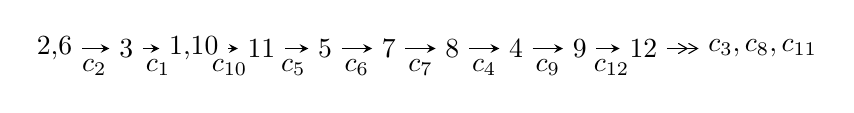
\begin{tikzpicture}[x=23pt, y=7pt]
	% node
	\node (A0) at (-1/8, 0) {2,6};
	\node (A1) at (1, 0) {3};
	\node (A2) at (33/16, 0) {1,10};
	\node (A3) at (25/8, 0) {11};
	\node (A4) at (33/8, 0) {5};
	\node (A5) at (41/8, 0) {7};
	\node (A6) at (49/8, 0) {8};
	\node (A7) at (57/8, 0) {4};
	\node (A8) at (65/8, 0) {9};
	\node (A9) at (73/8, 0) {12};
	\node (C1) at (1/2, -1) {$c_{2}$};
	\node (C2) at (3/2, -1) {$c_{1}$};
	\node (C3) at (21/8, -1) {$c_{10}$};
	\node (C4) at (29/8, -1) {$c_{5}$};
	\node (C5) at (37/8, -1) {$c_{6}$};
	\node (C6) at (45/8, -1) {$c_{7}$};
	\node (C7) at (53/8, -1) {$c_{4}$};
	\node (C8) at (61/8, -1) {$c_{9}$};
	\node (C9) at (69/8, -1) {$c_{12}$};
	\node (A10) at (11, 0) {$c_{3},c_{8},c_{11}$};

	% edge
	\draw[->,>=stealth]	
	(A0) edge (A1) (A1) edge (A2) (A2) edge (A3) (A3) edge (A4) (A4) edge (A5) (A5) edge (A6) (A6) edge (A7) (A7) edge (A8) (A8) edge (A9) ;
	\draw[->>,>={angle 60}]	
	(A9) edge (A10);
\end{tikzpicture} \\ 

\end{tabular} \\

\footnotetext{
The image of knot diagram is generated by the software ``\textbf{Draw programme}" developed by Andrew Bartholomew(\url{http://www.layer8.co.uk/maths/draw/index.htm\#Running-draw}), where we modified some parts for our purpose(\url{https://github.com/CATsTAILs/LinksPainter}).
}\phantom \\ \newline 
\centering \textbf{Ideals for irreducible components\footnotemark of $X_{\text{par}}$} 
 
\begin{align*}
I^u_{1}&=\langle 
42 u^{95}-107 u^{94}+\cdots+4 b+15,\;8 u^{95}-5 u^{94}+\cdots+4 a-3,\;u^{96}-4 u^{95}+\cdots+2 u-1\rangle \\
I^u_{2}&=\langle 
b- a,\;u^2 a+a^2+a u+u^2+a+u+1,\;u^3+u^2-1\rangle \\
I^u_{3}&=\langle 
b-1,\;a-1,\;u^3+u^2-1\rangle \\
\\
\end{align*}
\raggedright * 3 irreducible components of $\dim_{\mathbb{C}}=0$, with total 105 representations.\\
\footnotetext{All coefficients of polynomials are rational numbers. But the coefficients are sometimes approximated in decimal forms when there is not enough margin.}
\newpage
\renewcommand{\arraystretch}{1}
\centering \section*{I. $I^u_{1}= \langle 42 u^{95}-107 u^{94}+\cdots+4 b+15,\;8 u^{95}-5 u^{94}+\cdots+4 a-3,\;u^{96}-4 u^{95}+\cdots+2 u-1 \rangle$}
\flushleft \textbf{(i) Arc colorings}\\
\begin{tabular}{m{7pt} m{180pt} m{7pt} m{180pt} }
\flushright $a_{2}=$&$\begin{pmatrix}1\\0\end{pmatrix}$ \\
\flushright $a_{6}=$&$\begin{pmatrix}0\\u\end{pmatrix}$ \\
\flushright $a_{3}=$&$\begin{pmatrix}1\\u^2\end{pmatrix}$ \\
\flushright $a_{1}=$&$\begin{pmatrix}- u^2+1\\- u^4\end{pmatrix}$ \\
\flushright $a_{10}=$&$\begin{pmatrix}-2 u^{95}+\frac{5}{4} u^{94}+\cdots+\frac{3}{4} u+\frac{3}{4}\\-10.5000 u^{95}+26.7500 u^{94}+\cdots+7.75000 u-3.75000\end{pmatrix}$ \\
\flushright $a_{11}=$&$\begin{pmatrix}-3.75000 u^{95}+14.5000 u^{94}+\cdots+7.25000 u-4.75000\\-\frac{7}{4} u^{95}+\frac{17}{2} u^{94}+\cdots+\frac{11}{4} u-4\end{pmatrix}$ \\
\flushright $a_{5}=$&$\begin{pmatrix}u\\u\end{pmatrix}$ \\
\flushright $a_{7}=$&$\begin{pmatrix}- u^3\\- u^3+u\end{pmatrix}$ \\
\flushright $a_{8}=$&$\begin{pmatrix}\frac{1}{4} u^{93}-\frac{3}{4} u^{92}+\cdots-\frac{7}{2} u+\frac{3}{4}\\\frac{1}{4} u^{95}-\frac{3}{4} u^{94}+\cdots-\frac{15}{2} u^3+\frac{15}{4} u^2\end{pmatrix}$ \\
\flushright $a_{4}=$&$\begin{pmatrix}- u^8+u^6- u^4+1\\- u^8+2 u^6-2 u^4+2 u^2\end{pmatrix}$ \\
\flushright $a_{9}=$&$\begin{pmatrix}4 u^{95}-\frac{57}{4} u^{94}+\cdots-\frac{19}{4} u+\frac{21}{4}\\\frac{1}{2} u^{95}-\frac{19}{4} u^{94}+\cdots-\frac{11}{4} u+\frac{15}{4}\end{pmatrix}$ \\
\flushright $a_{12}=$&$\begin{pmatrix}-\frac{11}{4} u^{95}+\frac{43}{4} u^{94}+\cdots+5 u-\frac{11}{4}\\\frac{13}{4} u^{95}-\frac{29}{4} u^{94}+\cdots+\frac{5}{4} u^2-\frac{5}{2} u\end{pmatrix}$\\&\end{tabular}
\flushleft \textbf{(ii) Obstruction class $= -1$}\\~\\
\flushleft \textbf{(iii) Cusp Shapes $= \frac{11}{4} u^{95}+\frac{3}{2} u^{94}+\cdots-\frac{29}{4} u-\frac{13}{2}$}\\~\\
\newpage\renewcommand{\arraystretch}{1}
\flushleft \textbf{(iv) u-Polynomials at the component}\newline \\
\begin{tabular}{m{50pt}|m{274pt}}
Crossings & \hspace{64pt}u-Polynomials at each crossing \\
\hline $$\begin{aligned}c_{1},c_{6}\end{aligned}$$&$\begin{aligned}
&u^{96}+32 u^{95}+\cdots-6 u+1
\end{aligned}$\\
\hline $$\begin{aligned}c_{2},c_{5}\end{aligned}$$&$\begin{aligned}
&u^{96}+4 u^{95}+\cdots-2 u-1
\end{aligned}$\\
\hline $$\begin{aligned}c_{3}\end{aligned}$$&$\begin{aligned}
&u^{96}-4 u^{95}+\cdots+348300 u-31428
\end{aligned}$\\
\hline $$\begin{aligned}c_{4},c_{9}\end{aligned}$$&$\begin{aligned}
&u^{96}- u^{95}+\cdots+512 u+512
\end{aligned}$\\
\hline $$\begin{aligned}c_{7}\end{aligned}$$&$\begin{aligned}
&u^{96}-4 u^{95}+\cdots-1638 u-193
\end{aligned}$\\
\hline $$\begin{aligned}c_{8},c_{11},c_{12}\end{aligned}$$&$\begin{aligned}
&u^{96}+4 u^{95}+\cdots-10 u-1
\end{aligned}$\\
\hline $$\begin{aligned}c_{10}\end{aligned}$$&$\begin{aligned}
&u^{96}+20 u^{95}+\cdots-142864 u+20513
\end{aligned}$\\
\hline
\end{tabular}\\~\\
\newpage\renewcommand{\arraystretch}{1}
\flushleft \textbf{(v) Riley Polynomials at the component}\newline \\
\begin{tabular}{m{50pt}|m{274pt}}
Crossings & \hspace{64pt}Riley Polynomials at each crossing \\
\hline $$\begin{aligned}c_{1},c_{6}\end{aligned}$$&$\begin{aligned}
&y^{96}+68 y^{95}+\cdots+6 y+1
\end{aligned}$\\
\hline $$\begin{aligned}c_{2},c_{5}\end{aligned}$$&$\begin{aligned}
&y^{96}-32 y^{95}+\cdots+6 y+1
\end{aligned}$\\
\hline $$\begin{aligned}c_{3}\end{aligned}$$&$\begin{aligned}
&y^{96}-16 y^{95}+\cdots-14375034360 y+987719184
\end{aligned}$\\
\hline $$\begin{aligned}c_{4},c_{9}\end{aligned}$$&$\begin{aligned}
&y^{96}-49 y^{95}+\cdots-5898240 y+262144
\end{aligned}$\\
\hline $$\begin{aligned}c_{7}\end{aligned}$$&$\begin{aligned}
&y^{96}+8 y^{95}+\cdots-678546 y+37249
\end{aligned}$\\
\hline $$\begin{aligned}c_{8},c_{11},c_{12}\end{aligned}$$&$\begin{aligned}
&y^{96}+88 y^{95}+\cdots-50 y+1
\end{aligned}$\\
\hline $$\begin{aligned}c_{10}\end{aligned}$$&$\begin{aligned}
&y^{96}+36 y^{95}+\cdots-203007043282 y+420783169
\end{aligned}$\\
\hline
\end{tabular}\\~\\
\newpage\flushleft \textbf{(vi) Complex Volumes and Cusp Shapes}
$$\begin{array}{c|c|c}  
\text{Solutions to }I^u_{1}& \I (\text{vol} + \sqrt{-1}CS) & \text{Cusp shape}\\
 \hline 
\begin{aligned}
u &= -0.673892 + 0.747342 I \\
a &= \phantom{-}0.35572 + 1.82806 I \\
b &= \phantom{-}1.40911 + 1.47675 I\end{aligned}
 & -1.96032 - 4.54873 I & \phantom{-0.000000 } 0 \\ \hline\begin{aligned}
u &= -0.673892 - 0.747342 I \\
a &= \phantom{-}0.35572 - 1.82806 I \\
b &= \phantom{-}1.40911 - 1.47675 I\end{aligned}
 & -1.96032 + 4.54873 I & \phantom{-0.000000 } 0 \\ \hline\begin{aligned}
u &= \phantom{-}0.610514 + 0.800542 I \\
a &= -1.56996 + 0.96365 I \\
b &= -1.181540 - 0.299685 I\end{aligned}
 & -6.80579 + 1.30564 I & \phantom{-0.000000 } 0 \\ \hline\begin{aligned}
u &= \phantom{-}0.610514 - 0.800542 I \\
a &= -1.56996 - 0.96365 I \\
b &= -1.181540 + 0.299685 I\end{aligned}
 & -6.80579 - 1.30564 I & \phantom{-0.000000 } 0 \\ \hline\begin{aligned}
u &= \phantom{-}0.979747 + 0.046907 I \\
a &= \phantom{-}0.155311 - 0.922681 I \\
b &= \phantom{-}0.0381284 + 0.0275714 I\end{aligned}
 & -1.98868 - 1.54484 I & \phantom{-0.000000 } 0 \\ \hline\begin{aligned}
u &= \phantom{-}0.979747 - 0.046907 I \\
a &= \phantom{-}0.155311 + 0.922681 I \\
b &= \phantom{-}0.0381284 - 0.0275714 I\end{aligned}
 & -1.98868 + 1.54484 I & \phantom{-0.000000 } 0 \\ \hline\begin{aligned}
u &= -0.709327 + 0.742547 I \\
a &= -0.28755 - 1.74215 I \\
b &= -1.25847 - 1.44166 I\end{aligned}
 & \phantom{-}3.38377 - 1.26164 I & \phantom{-0.000000 } 0 \\ \hline\begin{aligned}
u &= -0.709327 - 0.742547 I \\
a &= -0.28755 + 1.74215 I \\
b &= -1.25847 + 1.44166 I\end{aligned}
 & \phantom{-}3.38377 + 1.26164 I & \phantom{-0.000000 } 0 \\ \hline\begin{aligned}
u &= -0.967386 + 0.065292 I \\
a &= -1.229590 - 0.581737 I \\
b &= -2.15051 - 0.41869 I\end{aligned}
 & -4.83200 + 3.64059 I & \phantom{-0.000000 } 0 \\ \hline\begin{aligned}
u &= -0.967386 - 0.065292 I \\
a &= -1.229590 + 0.581737 I \\
b &= -2.15051 + 0.41869 I\end{aligned}
 & -4.83200 - 3.64059 I & \phantom{-0.000000 } 0\\
 \hline 
 \end{array}$$\newpage$$\begin{array}{c|c|c}  
\text{Solutions to }I^u_{1}& \I (\text{vol} + \sqrt{-1}CS) & \text{Cusp shape}\\
 \hline 
\begin{aligned}
u &= \phantom{-}1.030310 + 0.051234 I \\
a &= -0.193028 + 1.096310 I \\
b &= -0.0651951 + 0.0213549 I\end{aligned}
 & -7.53067 - 4.37669 I & \phantom{-0.000000 } 0 \\ \hline\begin{aligned}
u &= \phantom{-}1.030310 - 0.051234 I \\
a &= -0.193028 - 1.096310 I \\
b &= -0.0651951 - 0.0213549 I\end{aligned}
 & -7.53067 + 4.37669 I & \phantom{-0.000000 } 0 \\ \hline\begin{aligned}
u &= \phantom{-}0.733394 + 0.726335 I \\
a &= -0.95055 + 1.72774 I \\
b &= -0.647889 + 0.840039 I\end{aligned}
 & \phantom{-}3.78669 - 0.46878 I & \phantom{-0.000000 } 0 \\ \hline\begin{aligned}
u &= \phantom{-}0.733394 - 0.726335 I \\
a &= -0.95055 - 1.72774 I \\
b &= -0.647889 - 0.840039 I\end{aligned}
 & \phantom{-}3.78669 + 0.46878 I & \phantom{-0.000000 } 0 \\ \hline\begin{aligned}
u &= \phantom{-}0.659051 + 0.798621 I \\
a &= \phantom{-}1.60539 - 1.26651 I \\
b &= \phantom{-}1.319350 - 0.083707 I\end{aligned}
 & -0.15569 + 3.01549 I & \phantom{-0.000000 } 0 \\ \hline\begin{aligned}
u &= \phantom{-}0.659051 - 0.798621 I \\
a &= \phantom{-}1.60539 + 1.26651 I \\
b &= \phantom{-}1.319350 + 0.083707 I\end{aligned}
 & -0.15569 - 3.01549 I & \phantom{-0.000000 } 0 \\ \hline\begin{aligned}
u &= \phantom{-}0.762531 + 0.701280 I \\
a &= \phantom{-}0.57033 - 1.80163 I \\
b &= \phantom{-}0.232663 - 1.020810 I\end{aligned}
 & -0.63753 - 4.16046 I & \phantom{-0.000000 } 0 \\ \hline\begin{aligned}
u &= \phantom{-}0.762531 - 0.701280 I \\
a &= \phantom{-}0.57033 + 1.80163 I \\
b &= \phantom{-}0.232663 + 1.020810 I\end{aligned}
 & -0.63753 + 4.16046 I & \phantom{-0.000000 } 0 \\ \hline\begin{aligned}
u &= -0.960082\phantom{ +0.000000I} \\
a &= \phantom{-}1.35659\phantom{ +0.000000I} \\
b &= \phantom{-}2.25623\phantom{ +0.000000I}\end{aligned}
 & -1.13345\phantom{ +0.000000I} & \phantom{-0.000000 } 0 \\ \hline\begin{aligned}
u &= \phantom{-}0.707856 + 0.762895 I \\
a &= \phantom{-}1.32470 - 1.62047 I \\
b &= \phantom{-}1.068090 - 0.609735 I\end{aligned}
 & \phantom{-}0.77305 + 3.23760 I & \phantom{-0.000000 } 0\\
 \hline 
 \end{array}$$\newpage$$\begin{array}{c|c|c}  
\text{Solutions to }I^u_{1}& \I (\text{vol} + \sqrt{-1}CS) & \text{Cusp shape}\\
 \hline 
\begin{aligned}
u &= \phantom{-}0.707856 - 0.762895 I \\
a &= \phantom{-}1.32470 + 1.62047 I \\
b &= \phantom{-}1.068090 + 0.609735 I\end{aligned}
 & \phantom{-}0.77305 - 3.23760 I & \phantom{-0.000000 } 0 \\ \hline\begin{aligned}
u &= -0.775850 + 0.699755 I \\
a &= \phantom{-}0.36075 + 1.44555 I \\
b &= \phantom{-}1.10144 + 1.11306 I\end{aligned}
 & \phantom{-}2.18338 + 1.93521 I & \phantom{-0.000000 } 0 \\ \hline\begin{aligned}
u &= -0.775850 - 0.699755 I \\
a &= \phantom{-}0.36075 - 1.44555 I \\
b &= \phantom{-}1.10144 - 1.11306 I\end{aligned}
 & \phantom{-}2.18338 - 1.93521 I & \phantom{-0.000000 } 0 \\ \hline\begin{aligned}
u &= \phantom{-}0.665389 + 0.826895 I \\
a &= -1.81218 + 1.28162 I \\
b &= -1.59046 + 0.04424 I\end{aligned}
 & \phantom{-}1.13562 + 7.07104 I & \phantom{-0.000000 } 0 \\ \hline\begin{aligned}
u &= \phantom{-}0.665389 - 0.826895 I \\
a &= -1.81218 - 1.28162 I \\
b &= -1.59046 - 0.04424 I\end{aligned}
 & \phantom{-}1.13562 - 7.07104 I & \phantom{-0.000000 } 0 \\ \hline\begin{aligned}
u &= -0.730626 + 0.577652 I \\
a &= -0.65546 - 1.66699 I \\
b &= -1.44919 - 1.07027 I\end{aligned}
 & -3.32770 + 3.63559 I & \phantom{-0.000000 } 0 \\ \hline\begin{aligned}
u &= -0.730626 - 0.577652 I \\
a &= -0.65546 + 1.66699 I \\
b &= -1.44919 + 1.07027 I\end{aligned}
 & -3.32770 - 3.63559 I & \phantom{-0.000000 } 0 \\ \hline\begin{aligned}
u &= \phantom{-}0.660642 + 0.842059 I \\
a &= \phantom{-}1.91437 - 1.22201 I \\
b &= \phantom{-}1.70662 + 0.06127 I\end{aligned}
 & -4.43080 + 10.74230 I & \phantom{-0.000000 } 0 \\ \hline\begin{aligned}
u &= \phantom{-}0.660642 - 0.842059 I \\
a &= \phantom{-}1.91437 + 1.22201 I \\
b &= \phantom{-}1.70662 - 0.06127 I\end{aligned}
 & -4.43080 - 10.74230 I & \phantom{-0.000000 } 0 \\ \hline\begin{aligned}
u &= \phantom{-}0.901488 + 0.213540 I \\
a &= -0.510275 + 0.624002 I \\
b &= -0.020787 - 0.184467 I\end{aligned}
 & -4.26322 - 0.28528 I & \phantom{-0.000000 } 0\\
 \hline 
 \end{array}$$\newpage$$\begin{array}{c|c|c}  
\text{Solutions to }I^u_{1}& \I (\text{vol} + \sqrt{-1}CS) & \text{Cusp shape}\\
 \hline 
\begin{aligned}
u &= \phantom{-}0.901488 - 0.213540 I \\
a &= -0.510275 - 0.624002 I \\
b &= -0.020787 + 0.184467 I\end{aligned}
 & -4.26322 + 0.28528 I & \phantom{-0.000000 } 0 \\ \hline\begin{aligned}
u &= -1.073080 + 0.099941 I \\
a &= -0.410079 - 0.769436 I \\
b &= -1.58578 - 0.51734 I\end{aligned}
 & -6.36389 + 2.68095 I & \phantom{-0.000000 } 0 \\ \hline\begin{aligned}
u &= -1.073080 - 0.099941 I \\
a &= -0.410079 + 0.769436 I \\
b &= -1.58578 + 0.51734 I\end{aligned}
 & -6.36389 - 2.68095 I & \phantom{-0.000000 } 0 \\ \hline\begin{aligned}
u &= -1.083550 + 0.131554 I \\
a &= \phantom{-}0.347074 + 0.994674 I \\
b &= \phantom{-}1.54158 + 0.66296 I\end{aligned}
 & -5.41947 + 6.78456 I & \phantom{-0.000000 } 0 \\ \hline\begin{aligned}
u &= -1.083550 - 0.131554 I \\
a &= \phantom{-}0.347074 - 0.994674 I \\
b &= \phantom{-}1.54158 - 0.66296 I\end{aligned}
 & -5.41947 - 6.78456 I & \phantom{-0.000000 } 0 \\ \hline\begin{aligned}
u &= -0.784865 + 0.781046 I \\
a &= -0.09778 + 1.55559 I \\
b &= \phantom{-}0.73470 + 1.51372 I\end{aligned}
 & \phantom{-}1.86446 + 1.37751 I & \phantom{-0.000000 } 0 \\ \hline\begin{aligned}
u &= -0.784865 - 0.781046 I \\
a &= -0.09778 - 1.55559 I \\
b &= \phantom{-}0.73470 - 1.51372 I\end{aligned}
 & \phantom{-}1.86446 - 1.37751 I & \phantom{-0.000000 } 0 \\ \hline\begin{aligned}
u &= -1.105400 + 0.077234 I \\
a &= \phantom{-}0.162873 + 0.610352 I \\
b &= \phantom{-}1.42379 + 0.40984 I\end{aligned}
 & -12.97280 + 0.50568 I & \phantom{-0.000000 } 0 \\ \hline\begin{aligned}
u &= -1.105400 - 0.077234 I \\
a &= \phantom{-}0.162873 - 0.610352 I \\
b &= \phantom{-}1.42379 - 0.40984 I\end{aligned}
 & -12.97280 - 0.50568 I & \phantom{-0.000000 } 0 \\ \hline\begin{aligned}
u &= \phantom{-}0.988693 + 0.501263 I \\
a &= \phantom{-}0.452510 + 0.076254 I \\
b &= -0.413738 + 0.804553 I\end{aligned}
 & -3.24273 + 0.34411 I & \phantom{-0.000000 } 0\\
 \hline 
 \end{array}$$\newpage$$\begin{array}{c|c|c}  
\text{Solutions to }I^u_{1}& \I (\text{vol} + \sqrt{-1}CS) & \text{Cusp shape}\\
 \hline 
\begin{aligned}
u &= \phantom{-}0.988693 - 0.501263 I \\
a &= \phantom{-}0.452510 - 0.076254 I \\
b &= -0.413738 - 0.804553 I\end{aligned}
 & -3.24273 - 0.34411 I & \phantom{-0.000000 } 0 \\ \hline\begin{aligned}
u &= -1.101930 + 0.141181 I \\
a &= -0.228488 - 1.073210 I \\
b &= -1.46508 - 0.71255 I\end{aligned}
 & -11.1619 + 10.3484 I & \phantom{-0.000000 } 0 \\ \hline\begin{aligned}
u &= -1.101930 - 0.141181 I \\
a &= -0.228488 + 1.073210 I \\
b &= -1.46508 + 0.71255 I\end{aligned}
 & -11.1619 - 10.3484 I & \phantom{-0.000000 } 0 \\ \hline\begin{aligned}
u &= \phantom{-}1.022000 + 0.483742 I \\
a &= -0.668093 - 0.127010 I \\
b &= \phantom{-}0.240155 - 0.912102 I\end{aligned}
 & -9.09474 + 3.58525 I & \phantom{-0.000000 } 0 \\ \hline\begin{aligned}
u &= \phantom{-}1.022000 - 0.483742 I \\
a &= -0.668093 + 0.127010 I \\
b &= \phantom{-}0.240155 + 0.912102 I\end{aligned}
 & -9.09474 - 3.58525 I & \phantom{-0.000000 } 0 \\ \hline\begin{aligned}
u &= \phantom{-}0.992459 + 0.552581 I \\
a &= -0.194835 - 0.315236 I \\
b &= \phantom{-}0.706176 - 0.947524 I\end{aligned}
 & -3.69107 - 3.59998 I & \phantom{-0.000000 } 0 \\ \hline\begin{aligned}
u &= \phantom{-}0.992459 - 0.552581 I \\
a &= -0.194835 + 0.315236 I \\
b &= \phantom{-}0.706176 + 0.947524 I\end{aligned}
 & -3.69107 + 3.59998 I & \phantom{-0.000000 } 0 \\ \hline\begin{aligned}
u &= -0.968160 + 0.632527 I \\
a &= -1.44301 - 1.24978 I \\
b &= -1.86779 - 0.40200 I\end{aligned}
 & -4.11887 + 1.23703 I & \phantom{-0.000000 } 0 \\ \hline\begin{aligned}
u &= -0.968160 - 0.632527 I \\
a &= -1.44301 + 1.24978 I \\
b &= -1.86779 + 0.40200 I\end{aligned}
 & -4.11887 - 1.23703 I & \phantom{-0.000000 } 0 \\ \hline\begin{aligned}
u &= -0.841043 + 0.799563 I \\
a &= \phantom{-}0.556872 - 1.272450 I \\
b &= -0.11791 - 1.48091 I\end{aligned}
 & \phantom{-}4.25951 + 3.93964 I & \phantom{-0.000000 } 0\\
 \hline 
 \end{array}$$\newpage$$\begin{array}{c|c|c}  
\text{Solutions to }I^u_{1}& \I (\text{vol} + \sqrt{-1}CS) & \text{Cusp shape}\\
 \hline 
\begin{aligned}
u &= -0.841043 - 0.799563 I \\
a &= \phantom{-}0.556872 + 1.272450 I \\
b &= -0.11791 + 1.48091 I\end{aligned}
 & \phantom{-}4.25951 - 3.93964 I & \phantom{-0.000000 } 0 \\ \hline\begin{aligned}
u &= -0.944916 + 0.675440 I \\
a &= \phantom{-}1.34304 + 0.90487 I \\
b &= \phantom{-}1.63244 + 0.15845 I\end{aligned}
 & \phantom{-}1.65341 + 3.36196 I & \phantom{-0.000000 } 0 \\ \hline\begin{aligned}
u &= -0.944916 - 0.675440 I \\
a &= \phantom{-}1.34304 - 0.90487 I \\
b &= \phantom{-}1.63244 - 0.15845 I\end{aligned}
 & \phantom{-}1.65341 - 3.36196 I & \phantom{-0.000000 } 0 \\ \hline\begin{aligned}
u &= \phantom{-}0.947334 + 0.676570 I \\
a &= \phantom{-}1.42444 - 0.49363 I \\
b &= \phantom{-}2.17942 - 0.77675 I\end{aligned}
 & -1.20862 - 1.14741 I & \phantom{-0.000000 } 0 \\ \hline\begin{aligned}
u &= \phantom{-}0.947334 - 0.676570 I \\
a &= \phantom{-}1.42444 + 0.49363 I \\
b &= \phantom{-}2.17942 + 0.77675 I\end{aligned}
 & -1.20862 + 1.14741 I & \phantom{-0.000000 } 0 \\ \hline\begin{aligned}
u &= \phantom{-}1.030590 + 0.564562 I \\
a &= \phantom{-}0.333144 + 0.623335 I \\
b &= -0.66234 + 1.25095 I\end{aligned}
 & -9.99197 - 6.19410 I & \phantom{-0.000000 } 0 \\ \hline\begin{aligned}
u &= \phantom{-}1.030590 - 0.564562 I \\
a &= \phantom{-}0.333144 - 0.623335 I \\
b &= -0.66234 - 1.25095 I\end{aligned}
 & -9.99197 + 6.19410 I & \phantom{-0.000000 } 0 \\ \hline\begin{aligned}
u &= -0.855816 + 0.821883 I \\
a &= -0.85261 + 1.35962 I \\
b &= -0.13500 + 1.71492 I\end{aligned}
 & -0.87177 + 6.94889 I & \phantom{-0.000000 } 0 \\ \hline\begin{aligned}
u &= -0.855816 - 0.821883 I \\
a &= -0.85261 - 1.35962 I \\
b &= -0.13500 - 1.71492 I\end{aligned}
 & -0.87177 - 6.94889 I & \phantom{-0.000000 } 0 \\ \hline\begin{aligned}
u &= \phantom{-}0.967510 + 0.689054 I \\
a &= -1.41955 + 0.95893 I \\
b &= -2.25006 + 1.18191 I\end{aligned}
 & \phantom{-}3.07239 - 4.95468 I & \phantom{-0.000000 } 0\\
 \hline 
 \end{array}$$\newpage$$\begin{array}{c|c|c}  
\text{Solutions to }I^u_{1}& \I (\text{vol} + \sqrt{-1}CS) & \text{Cusp shape}\\
 \hline 
\begin{aligned}
u &= \phantom{-}0.967510 - 0.689054 I \\
a &= -1.41955 - 0.95893 I \\
b &= -2.25006 - 1.18191 I\end{aligned}
 & \phantom{-}3.07239 + 4.95468 I & \phantom{-0.000000 } 0 \\ \hline\begin{aligned}
u &= -0.914722 + 0.776063 I \\
a &= -1.207680 + 0.382210 I \\
b &= -0.933874 + 0.933577 I\end{aligned}
 & \phantom{-}4.03238 + 1.96937 I & \phantom{-0.000000 } 0 \\ \hline\begin{aligned}
u &= -0.914722 - 0.776063 I \\
a &= -1.207680 - 0.382210 I \\
b &= -0.933874 - 0.933577 I\end{aligned}
 & \phantom{-}4.03238 - 1.96937 I & \phantom{-0.000000 } 0 \\ \hline\begin{aligned}
u &= -0.982519 + 0.693996 I \\
a &= -1.70891 - 0.82601 I \\
b &= -1.91060 + 0.06642 I\end{aligned}
 & \phantom{-}2.55755 + 6.74718 I & \phantom{-0.000000 } 0 \\ \hline\begin{aligned}
u &= -0.982519 - 0.693996 I \\
a &= -1.70891 + 0.82601 I \\
b &= -1.91060 - 0.06642 I\end{aligned}
 & \phantom{-}2.55755 - 6.74718 I & \phantom{-0.000000 } 0 \\ \hline\begin{aligned}
u &= -0.948900 + 0.743844 I \\
a &= \phantom{-}1.51810 + 0.20015 I \\
b &= \phantom{-}1.47656 - 0.53578 I\end{aligned}
 & \phantom{-}1.36634 + 4.37637 I & \phantom{-0.000000 } 0 \\ \hline\begin{aligned}
u &= -0.948900 - 0.743844 I \\
a &= \phantom{-}1.51810 - 0.20015 I \\
b &= \phantom{-}1.47656 + 0.53578 I\end{aligned}
 & \phantom{-}1.36634 - 4.37637 I & \phantom{-0.000000 } 0 \\ \hline\begin{aligned}
u &= \phantom{-}0.361572 + 0.704455 I \\
a &= -0.843864 + 0.401713 I \\
b &= \phantom{-}0.071734 - 0.899301 I\end{aligned}
 & -8.11236 + 1.49674 I & -7.32882 + 0. I\phantom{ +0.000000I} \\ \hline\begin{aligned}
u &= \phantom{-}0.361572 - 0.704455 I \\
a &= -0.843864 - 0.401713 I \\
b &= \phantom{-}0.071734 + 0.899301 I\end{aligned}
 & -8.11236 - 1.49674 I & -7.32882 + 0. I\phantom{ +0.000000I} \\ \hline\begin{aligned}
u &= \phantom{-}0.987429 + 0.702312 I \\
a &= \phantom{-}1.34748 - 1.39365 I \\
b &= \phantom{-}2.26197 - 1.56132 I\end{aligned}
 & -0.07409 - 8.80368 I & \phantom{-0.000000 } 0\\
 \hline 
 \end{array}$$\newpage$$\begin{array}{c|c|c}  
\text{Solutions to }I^u_{1}& \I (\text{vol} + \sqrt{-1}CS) & \text{Cusp shape}\\
 \hline 
\begin{aligned}
u &= \phantom{-}0.987429 - 0.702312 I \\
a &= \phantom{-}1.34748 + 1.39365 I \\
b &= \phantom{-}2.26197 + 1.56132 I\end{aligned}
 & -0.07409 + 8.80368 I & \phantom{-0.000000 } 0 \\ \hline\begin{aligned}
u &= -1.000220 + 0.688530 I \\
a &= \phantom{-}1.84068 + 0.93653 I \\
b &= \phantom{-}2.06857 - 0.02614 I\end{aligned}
 & -2.93811 + 10.02960 I & \phantom{-0.000000 } 0 \\ \hline\begin{aligned}
u &= -1.000220 - 0.688530 I \\
a &= \phantom{-}1.84068 - 0.93653 I \\
b &= \phantom{-}2.06857 + 0.02614 I\end{aligned}
 & -2.93811 - 10.02960 I & \phantom{-0.000000 } 0 \\ \hline\begin{aligned}
u &= -0.914517 + 0.802398 I \\
a &= \phantom{-}1.37299 - 0.73011 I \\
b &= \phantom{-}0.93505 - 1.33698 I\end{aligned}
 & -1.052600 - 0.890735 I & \phantom{-0.000000 } 0 \\ \hline\begin{aligned}
u &= -0.914517 - 0.802398 I \\
a &= \phantom{-}1.37299 + 0.73011 I \\
b &= \phantom{-}0.93505 + 1.33698 I\end{aligned}
 & -1.052600 + 0.890735 I & \phantom{-0.000000 } 0 \\ \hline\begin{aligned}
u &= \phantom{-}1.021260 + 0.706015 I \\
a &= \phantom{-}0.96299 - 1.80167 I \\
b &= \phantom{-}2.01958 - 1.97104 I\end{aligned}
 & -1.24695 - 8.68885 I & \phantom{-0.000000 } 0 \\ \hline\begin{aligned}
u &= \phantom{-}1.021260 - 0.706015 I \\
a &= \phantom{-}0.96299 + 1.80167 I \\
b &= \phantom{-}2.01958 + 1.97104 I\end{aligned}
 & -1.24695 + 8.68885 I & \phantom{-0.000000 } 0 \\ \hline\begin{aligned}
u &= \phantom{-}1.037260 + 0.689346 I \\
a &= -0.61941 + 1.75820 I \\
b &= -1.72572 + 2.00532 I\end{aligned}
 & -8.08056 - 6.91284 I & \phantom{-0.000000 } 0 \\ \hline\begin{aligned}
u &= \phantom{-}1.037260 - 0.689346 I \\
a &= -0.61941 - 1.75820 I \\
b &= -1.72572 - 2.00532 I\end{aligned}
 & -8.08056 + 6.91284 I & \phantom{-0.000000 } 0 \\ \hline\begin{aligned}
u &= \phantom{-}0.225872 + 0.712033 I \\
a &= \phantom{-}0.513021 - 0.360124 I \\
b &= -0.584992 + 0.987864 I\end{aligned}
 & -6.75618 - 7.81009 I & -5.15386 + 6.01462 I\\
 \hline 
 \end{array}$$\newpage$$\begin{array}{c|c|c}  
\text{Solutions to }I^u_{1}& \I (\text{vol} + \sqrt{-1}CS) & \text{Cusp shape}\\
 \hline 
\begin{aligned}
u &= \phantom{-}0.225872 - 0.712033 I \\
a &= \phantom{-}0.513021 + 0.360124 I \\
b &= -0.584992 - 0.987864 I\end{aligned}
 & -6.75618 + 7.81009 I & -5.15386 - 6.01462 I \\ \hline\begin{aligned}
u &= \phantom{-}1.028450 + 0.718935 I \\
a &= -0.99531 + 2.02785 I \\
b &= -2.09188 + 2.15005 I\end{aligned}
 & \phantom{-}0.03178 - 12.86460 I & \phantom{-0.000000 } 0 \\ \hline\begin{aligned}
u &= \phantom{-}1.028450 - 0.718935 I \\
a &= -0.99531 - 2.02785 I \\
b &= -2.09188 - 2.15005 I\end{aligned}
 & \phantom{-}0.03178 + 12.86460 I & \phantom{-0.000000 } 0 \\ \hline\begin{aligned}
u &= \phantom{-}1.036220 + 0.723225 I \\
a &= \phantom{-}0.93729 - 2.15016 I \\
b &= \phantom{-}2.07005 - 2.26190 I\end{aligned}
 & -5.5765 - 16.5912 I & \phantom{-0.000000 } 0 \\ \hline\begin{aligned}
u &= \phantom{-}1.036220 - 0.723225 I \\
a &= \phantom{-}0.93729 + 2.15016 I \\
b &= \phantom{-}2.07005 + 2.26190 I\end{aligned}
 & -5.5765 + 16.5912 I & \phantom{-0.000000 } 0 \\ \hline\begin{aligned}
u &= \phantom{-}0.229697 + 0.666464 I \\
a &= -0.546602 + 0.470321 I \\
b &= \phantom{-}0.553918 - 0.824154 I\end{aligned}
 & -1.13431 - 4.43613 I & -0.95866 + 6.40467 I \\ \hline\begin{aligned}
u &= \phantom{-}0.229697 - 0.666464 I \\
a &= -0.546602 - 0.470321 I \\
b &= \phantom{-}0.553918 + 0.824154 I\end{aligned}
 & -1.13431 + 4.43613 I & -0.95866 - 6.40467 I \\ \hline\begin{aligned}
u &= \phantom{-}0.315520 + 0.614484 I \\
a &= \phantom{-}0.723984 - 0.544838 I \\
b &= -0.295922 + 0.657422 I\end{aligned}
 & -1.97243 - 0.73691 I & -3.75682 + 0.03141 I \\ \hline\begin{aligned}
u &= \phantom{-}0.315520 - 0.614484 I \\
a &= \phantom{-}0.723984 + 0.544838 I \\
b &= -0.295922 - 0.657422 I\end{aligned}
 & -1.97243 + 0.73691 I & -3.75682 - 0.03141 I \\ \hline\begin{aligned}
u &= \phantom{-}0.670863\phantom{ +0.000000I} \\
a &= \phantom{-}0.469393\phantom{ +0.000000I} \\
b &= -0.0917950\phantom{ +0.000000I}\end{aligned}
 & -0.909292\phantom{ +0.000000I} & -11.8320\phantom{ +0.000000I}\\
 \hline 
 \end{array}$$\newpage$$\begin{array}{c|c|c}  
\text{Solutions to }I^u_{1}& \I (\text{vol} + \sqrt{-1}CS) & \text{Cusp shape}\\
 \hline 
\begin{aligned}
u &= \phantom{-}0.061427 + 0.478934 I \\
a &= \phantom{-}0.485445 - 1.043810 I \\
b &= -0.783729 + 0.192259 I\end{aligned}
 & -1.78729 - 2.06625 I & -0.29523 + 4.09574 I \\ \hline\begin{aligned}
u &= \phantom{-}0.061427 - 0.478934 I \\
a &= \phantom{-}0.485445 + 1.043810 I \\
b &= -0.783729 - 0.192259 I\end{aligned}
 & -1.78729 + 2.06625 I & -0.29523 - 4.09574 I \\ \hline\begin{aligned}
u &= -0.331467 + 0.296157 I \\
a &= -0.06815 - 2.09602 I \\
b &= -0.861174 - 0.827960 I\end{aligned}
 & -3.49051 + 3.35120 I & -0.14805 - 4.26611 I \\ \hline\begin{aligned}
u &= -0.331467 - 0.296157 I \\
a &= -0.06815 + 2.09602 I \\
b &= -0.861174 + 0.827960 I\end{aligned}
 & -3.49051 - 3.35120 I & -0.14805 + 4.26611 I \\ \hline\begin{aligned}
u &= -0.111425 + 0.299353 I \\
a &= -0.50854 + 1.82130 I \\
b &= \phantom{-}0.676320 + 0.324196 I\end{aligned}
 & \phantom{-}1.245250 + 0.530627 I & \phantom{-}6.10933 - 1.75100 I \\ \hline\begin{aligned}
u &= -0.111425 - 0.299353 I \\
a &= -0.50854 - 1.82130 I \\
b &= \phantom{-}0.676320 - 0.324196 I\end{aligned}
 & \phantom{-}1.245250 - 0.530627 I & \phantom{-}6.10933 + 1.75100 I\\
 \hline 
 \end{array}$$\newpage\newpage\renewcommand{\arraystretch}{1}
\centering \section*{II. $I^u_{2}= \langle b- a,\;u^2 a+a^2+a u+u^2+a+u+1,\;u^3+u^2-1 \rangle$}
\flushleft \textbf{(i) Arc colorings}\\
\begin{tabular}{m{7pt} m{180pt} m{7pt} m{180pt} }
\flushright $a_{2}=$&$\begin{pmatrix}1\\0\end{pmatrix}$ \\
\flushright $a_{6}=$&$\begin{pmatrix}0\\u\end{pmatrix}$ \\
\flushright $a_{3}=$&$\begin{pmatrix}1\\u^2\end{pmatrix}$ \\
\flushright $a_{1}=$&$\begin{pmatrix}- u^2+1\\- u^2- u+1\end{pmatrix}$ \\
\flushright $a_{10}=$&$\begin{pmatrix}a\\a\end{pmatrix}$ \\
\flushright $a_{11}=$&$\begin{pmatrix}u^2 a+a u\\a u\end{pmatrix}$ \\
\flushright $a_{5}=$&$\begin{pmatrix}u\\u\end{pmatrix}$ \\
\flushright $a_{7}=$&$\begin{pmatrix}u^2-1\\u^2+u-1\end{pmatrix}$ \\
\flushright $a_{8}=$&$\begin{pmatrix}- u^2 a- a u- a- u-2\\- u^2 a- a u-1\end{pmatrix}$ \\
\flushright $a_{4}=$&$\begin{pmatrix}u\\u\end{pmatrix}$ \\
\flushright $a_{9}=$&$\begin{pmatrix}a\\a\end{pmatrix}$ \\
\flushright $a_{12}=$&$\begin{pmatrix}u^2 a- u^2- a-2 u-1\\- u^2- a-2 u-1\end{pmatrix}$\\&\end{tabular}
\flushleft \textbf{(ii) Obstruction class $= 1$}\\~\\
\flushleft \textbf{(iii) Cusp Shapes $= - u^2 a+a u- a-5 u-5$}\\~\\
\newpage\renewcommand{\arraystretch}{1}
\flushleft \textbf{(iv) u-Polynomials at the component}\newline \\
\begin{tabular}{m{50pt}|m{274pt}}
Crossings & \hspace{64pt}u-Polynomials at each crossing \\
\hline $$\begin{aligned}c_{1},c_{3},c_{11}\\c_{12}\end{aligned}$$&$\begin{aligned}
&(u^3- u^2+2 u-1)^2
\end{aligned}$\\
\hline $$\begin{aligned}c_{2}\end{aligned}$$&$\begin{aligned}
&(u^3+u^2-1)^2
\end{aligned}$\\
\hline $$\begin{aligned}c_{4},c_{9}\end{aligned}$$&$\begin{aligned}
&u^6
\end{aligned}$\\
\hline $$\begin{aligned}c_{5},c_{7},c_{10}\end{aligned}$$&$\begin{aligned}
&(u^3- u^2+1)^2
\end{aligned}$\\
\hline $$\begin{aligned}c_{6},c_{8}\end{aligned}$$&$\begin{aligned}
&(u^3+u^2+2 u+1)^2
\end{aligned}$\\
\hline
\end{tabular}\\~\\
\newpage\renewcommand{\arraystretch}{1}
\flushleft \textbf{(v) Riley Polynomials at the component}\newline \\
\begin{tabular}{m{50pt}|m{274pt}}
Crossings & \hspace{64pt}Riley Polynomials at each crossing \\
\hline $$\begin{aligned}c_{1},c_{3},c_{6}\\c_{8},c_{11},c_{12}\end{aligned}$$&$\begin{aligned}
&(y^3+3 y^2+2 y-1)^2
\end{aligned}$\\
\hline $$\begin{aligned}c_{2},c_{5},c_{7}\\c_{10}\end{aligned}$$&$\begin{aligned}
&(y^3- y^2+2 y-1)^2
\end{aligned}$\\
\hline $$\begin{aligned}c_{4},c_{9}\end{aligned}$$&$\begin{aligned}
&y^6
\end{aligned}$\\
\hline
\end{tabular}\\~\\
\newpage\flushleft \textbf{(vi) Complex Volumes and Cusp Shapes}
$$\begin{array}{c|c|c}  
\text{Solutions to }I^u_{2}& \I (\text{vol} + \sqrt{-1}CS) & \text{Cusp shape}\\
 \hline 
\begin{aligned}
u &= -0.877439 + 0.744862 I \\
a &= \phantom{-}0.162359 + 0.986732 I \\
b &= \phantom{-}0.162359 + 0.986732 I\end{aligned}
 & \phantom{-0.000000 -}5.65624 I & -2.97732 - 5.45590 I \\ \hline\begin{aligned}
u &= -0.877439 + 0.744862 I \\
a &= -0.500000 - 0.424452 I \\
b &= -0.500000 - 0.424452 I\end{aligned}
 & \phantom{-}4.13758 + 2.82812 I & \phantom{-}1.30443 - 3.86214 I \\ \hline\begin{aligned}
u &= -0.877439 - 0.744862 I \\
a &= \phantom{-}0.162359 - 0.986732 I \\
b &= \phantom{-}0.162359 - 0.986732 I\end{aligned}
 & \phantom{-0.000000 } -5.65624 I & -2.97732 + 5.45590 I \\ \hline\begin{aligned}
u &= -0.877439 - 0.744862 I \\
a &= -0.500000 + 0.424452 I \\
b &= -0.500000 + 0.424452 I\end{aligned}
 & \phantom{-}4.13758 - 2.82812 I & \phantom{-}1.30443 + 3.86214 I \\ \hline\begin{aligned}
u &= \phantom{-}0.754878\phantom{ +0.000000I} \\
a &= -1.16236 + 0.98673 I \\
b &= -1.16236 + 0.98673 I\end{aligned}
 & -4.13758 - 2.82812 I & -7.82711 - 0.80415 I \\ \hline\begin{aligned}
u &= \phantom{-}0.754878\phantom{ +0.000000I} \\
a &= -1.16236 - 0.98673 I \\
b &= -1.16236 - 0.98673 I\end{aligned}
 & -4.13758 + 2.82812 I & -7.82711 + 0.80415 I\\
 \hline 
 \end{array}$$\newpage\newpage\renewcommand{\arraystretch}{1}
\centering \section*{III. $I^u_{3}= \langle b-1,\;a-1,\;u^3+u^2-1 \rangle$}
\flushleft \textbf{(i) Arc colorings}\\
\begin{tabular}{m{7pt} m{180pt} m{7pt} m{180pt} }
\flushright $a_{2}=$&$\begin{pmatrix}1\\0\end{pmatrix}$ \\
\flushright $a_{6}=$&$\begin{pmatrix}0\\u\end{pmatrix}$ \\
\flushright $a_{3}=$&$\begin{pmatrix}1\\u^2\end{pmatrix}$ \\
\flushright $a_{1}=$&$\begin{pmatrix}- u^2+1\\- u^2- u+1\end{pmatrix}$ \\
\flushright $a_{10}=$&$\begin{pmatrix}1\\1\end{pmatrix}$ \\
\flushright $a_{11}=$&$\begin{pmatrix}u^2+u\\u\end{pmatrix}$ \\
\flushright $a_{5}=$&$\begin{pmatrix}u\\u\end{pmatrix}$ \\
\flushright $a_{7}=$&$\begin{pmatrix}u^2-1\\u^2+u-1\end{pmatrix}$ \\
\flushright $a_{8}=$&$\begin{pmatrix}u^2\\2 u^2+u-1\end{pmatrix}$ \\
\flushright $a_{4}=$&$\begin{pmatrix}u\\u\end{pmatrix}$ \\
\flushright $a_{9}=$&$\begin{pmatrix}1\\1\end{pmatrix}$ \\
\flushright $a_{12}=$&$\begin{pmatrix}u\\- u^2+u\end{pmatrix}$\\&\end{tabular}
\flushleft \textbf{(ii) Obstruction class $= 1$}\\~\\
\flushleft \textbf{(iii) Cusp Shapes $= u^2+u-1$}\\~\\
\newpage\renewcommand{\arraystretch}{1}
\flushleft \textbf{(iv) u-Polynomials at the component}\newline \\
\begin{tabular}{m{50pt}|m{274pt}}
Crossings & \hspace{64pt}u-Polynomials at each crossing \\
\hline $$\begin{aligned}c_{1},c_{3},c_{11}\\c_{12}\end{aligned}$$&$\begin{aligned}
&u^3- u^2+2 u-1
\end{aligned}$\\
\hline $$\begin{aligned}c_{2}\end{aligned}$$&$\begin{aligned}
&u^3+u^2-1
\end{aligned}$\\
\hline $$\begin{aligned}c_{4},c_{9}\end{aligned}$$&$\begin{aligned}
&u^3
\end{aligned}$\\
\hline $$\begin{aligned}c_{5},c_{7},c_{10}\end{aligned}$$&$\begin{aligned}
&u^3- u^2+1
\end{aligned}$\\
\hline $$\begin{aligned}c_{6},c_{8}\end{aligned}$$&$\begin{aligned}
&u^3+u^2+2 u+1
\end{aligned}$\\
\hline
\end{tabular}\\~\\
\newpage\renewcommand{\arraystretch}{1}
\flushleft \textbf{(v) Riley Polynomials at the component}\newline \\
\begin{tabular}{m{50pt}|m{274pt}}
Crossings & \hspace{64pt}Riley Polynomials at each crossing \\
\hline $$\begin{aligned}c_{1},c_{3},c_{6}\\c_{8},c_{11},c_{12}\end{aligned}$$&$\begin{aligned}
&y^3+3 y^2+2 y-1
\end{aligned}$\\
\hline $$\begin{aligned}c_{2},c_{5},c_{7}\\c_{10}\end{aligned}$$&$\begin{aligned}
&y^3- y^2+2 y-1
\end{aligned}$\\
\hline $$\begin{aligned}c_{4},c_{9}\end{aligned}$$&$\begin{aligned}
&y^3
\end{aligned}$\\
\hline
\end{tabular}\\~\\
\newpage\flushleft \textbf{(vi) Complex Volumes and Cusp Shapes}
$$\begin{array}{c|c|c}  
\text{Solutions to }I^u_{3}& \I (\text{vol} + \sqrt{-1}CS) & \text{Cusp shape}\\
 \hline 
\begin{aligned}
u &= -0.877439 + 0.744862 I \\
a &= \phantom{-}1.00000\phantom{ +0.000000I} \\
b &= \phantom{-}1.00000\phantom{ +0.000000I}\end{aligned}
 & \phantom{-0.000000 } 0 & -1.66236 - 0.56228 I \\ \hline\begin{aligned}
u &= -0.877439 - 0.744862 I \\
a &= \phantom{-}1.00000\phantom{ +0.000000I} \\
b &= \phantom{-}1.00000\phantom{ +0.000000I}\end{aligned}
 & \phantom{-0.000000 } 0 & -1.66236 + 0.56228 I \\ \hline\begin{aligned}
u &= \phantom{-}0.754878\phantom{ +0.000000I} \\
a &= \phantom{-}1.00000\phantom{ +0.000000I} \\
b &= \phantom{-}1.00000\phantom{ +0.000000I}\end{aligned}
 & \phantom{-0.000000 } 0 & \phantom{-}0.324720\phantom{ +0.000000I}\\
 \hline 
 \end{array}$$\newpage
\newpage\renewcommand{\arraystretch}{1}
\centering \section*{ IV. u-Polynomials}
\begin{tabular}{m{50pt}|m{274pt}}
Crossings & \hspace{64pt}u-Polynomials at each crossing \\
\hline $$\begin{aligned}c_{1}\end{aligned}$$&$\begin{aligned}
&((u^3- u^2+2 u-1)^3)(u^{96}+32 u^{95}+\cdots-6 u+1)
\end{aligned}$\\
\hline $$\begin{aligned}c_{2}\end{aligned}$$&$\begin{aligned}
&((u^3+u^2-1)^3)(u^{96}+4 u^{95}+\cdots-2 u-1)
\end{aligned}$\\
\hline $$\begin{aligned}c_{3}\end{aligned}$$&$\begin{aligned}
&((u^3- u^2+2 u-1)^3)(u^{96}-4 u^{95}+\cdots+348300 u-31428)
\end{aligned}$\\
\hline $$\begin{aligned}c_{4},c_{9}\end{aligned}$$&$\begin{aligned}
&u^9(u^{96}- u^{95}+\cdots+512 u+512)
\end{aligned}$\\
\hline $$\begin{aligned}c_{5}\end{aligned}$$&$\begin{aligned}
&((u^3- u^2+1)^3)(u^{96}+4 u^{95}+\cdots-2 u-1)
\end{aligned}$\\
\hline $$\begin{aligned}c_{6}\end{aligned}$$&$\begin{aligned}
&((u^3+u^2+2 u+1)^3)(u^{96}+32 u^{95}+\cdots-6 u+1)
\end{aligned}$\\
\hline $$\begin{aligned}c_{7}\end{aligned}$$&$\begin{aligned}
&((u^3- u^2+1)^3)(u^{96}-4 u^{95}+\cdots-1638 u-193)
\end{aligned}$\\
\hline $$\begin{aligned}c_{8}\end{aligned}$$&$\begin{aligned}
&((u^3+u^2+2 u+1)^3)(u^{96}+4 u^{95}+\cdots-10 u-1)
\end{aligned}$\\
\hline $$\begin{aligned}c_{10}\end{aligned}$$&$\begin{aligned}
&((u^3- u^2+1)^3)(u^{96}+20 u^{95}+\cdots-142864 u+20513)
\end{aligned}$\\
\hline $$\begin{aligned}c_{11},c_{12}\end{aligned}$$&$\begin{aligned}
&((u^3- u^2+2 u-1)^3)(u^{96}+4 u^{95}+\cdots-10 u-1)
\end{aligned}$\\
\hline
\end{tabular}\newpage\renewcommand{\arraystretch}{1}
\centering \section*{ V. Riley Polynomials}
\begin{tabular}{m{50pt}|m{274pt}}
Crossings & \hspace{64pt}Riley Polynomials at each crossing \\
\hline $$\begin{aligned}c_{1},c_{6}\end{aligned}$$&$\begin{aligned}
&((y^3+3 y^2+2 y-1)^3)(y^{96}+68 y^{95}+\cdots+6 y+1)
\end{aligned}$\\
\hline $$\begin{aligned}c_{2},c_{5}\end{aligned}$$&$\begin{aligned}
&((y^3- y^2+2 y-1)^3)(y^{96}-32 y^{95}+\cdots+6 y+1)
\end{aligned}$\\
\hline $$\begin{aligned}c_{3}\end{aligned}$$&$\begin{aligned}
&(y^3+3 y^2+2 y-1)^3\\
&\cdot(y^{96}-16 y^{95}+\cdots-14375034360 y+987719184)
\end{aligned}$\\
\hline $$\begin{aligned}c_{4},c_{9}\end{aligned}$$&$\begin{aligned}
&y^9(y^{96}-49 y^{95}+\cdots-5898240 y+262144)
\end{aligned}$\\
\hline $$\begin{aligned}c_{7}\end{aligned}$$&$\begin{aligned}
&((y^3- y^2+2 y-1)^3)(y^{96}+8 y^{95}+\cdots-678546 y+37249)
\end{aligned}$\\
\hline $$\begin{aligned}c_{8},c_{11},c_{12}\end{aligned}$$&$\begin{aligned}
&((y^3+3 y^2+2 y-1)^3)(y^{96}+88 y^{95}+\cdots-50 y+1)
\end{aligned}$\\
\hline $$\begin{aligned}c_{10}\end{aligned}$$&$\begin{aligned}
&(y^3- y^2+2 y-1)^3\\
&\cdot(y^{96}+36 y^{95}+\cdots-203007043282 y+420783169)
\end{aligned}$\\
\hline
\end{tabular}
\vskip 2pc
\end{document}